\documentclass[border=2]{standalone}
\usepackage{tikz}

\usetikzlibrary{shapes,arrows,arrows.meta,fit,positioning}

\begin{document}
\begin{tikzpicture}
    \node at (0,0) (C) {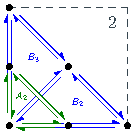
\includegraphics[scale=2]{overlap}};
    \node[left = of C] (A) {
        \begin{tabular}{c}
            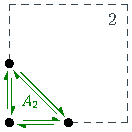
\includegraphics[scale=1.5]{A}  \\  
            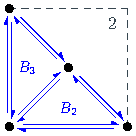
\includegraphics[scale=1.5]{B}
        \end{tabular}
    };
    \node[right = of C] (B) {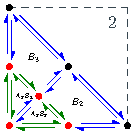
\includegraphics[scale=2]{splits}};
    
    \draw[very thick, -latex] (A) -- (C);
    \draw[very thick, -latex] (C) -- (B);
\end{tikzpicture}
\end{document}
